% En esta sección se presenta una breve descripción de la solución que se propone, 
% el principal objetivo de esta sección es poder dar el bosquejo de la solución 
% para que pueda ser evaluado. No es necesario detalles, pero sí mencionar sus 
% componentes generales. 
% Si las tecnologías que se van a utilizar ya están establecidas, se deberán 
% incluir aquí. De no estar definidas todas, enumerar las que sí están definidas 
% y explicar qué consideraciones tendrán en cuenta para definir las restantes.

\noindent Como respuesta a las problemáticas presentadas anteriormente nosotros desarrollamos una arquitectura
completamente distribuida, opuesta totalmente al modelo monolítico prevaleciente en la industria de los videojuegos. 
El estado del juego no se encuentra restringido a un único nodo servidor, sino que se encuentra 
distribuido en varios, cada uno con igual importancia y responsabilidades que el resto. El conjunto del estado en cada uno de estos nodos compone el 
estado del juego en su totalidad.

El aspecto central del videojuego desarrollado es el uso que hace del \textbf{modelo de actores}.
Dicho modelo se basa en el \textbf{actor} como mínima unidad de cómputo y el pasaje de \textbf{mensajes} como única manera
de compartir información entre los actores. En la práctica, esto significa que toda la lógica del juego
es procesada por los actores, y la comunicación entre ellos se realiza únicamente mediante mensajes.
Este paradigma, ideado por Carl Hewitt en los años 70, eliminá varios de los problemas presentes
en la programación concurrente tradicional que mencionamos anteriormente, como
los \textit{deadlocks} y \textit{race conditions}, al eliminar el uso de memoria compartida
como herramienta de comunicación en el sistema.
Este modelo además resulta en una forma natural de representar a las entidades del videojuego, donde podemos plantear una 
relación \textbf{1 a 1} entre entidad y actor. Si además establecemos que el estado de cada entidad 
debería ser administrado por ella misma, otra característica intrínseca del modelo de actores,
se desprende entonces que se ajusta perfectamente a lo que queremos desarrollar.

Existen muchas implementaciones del modelo de actores (el lenguaje \textit{Erlang} o el framework de 
\textit{Rust actix}) pero nosotros nos decantamos por \textit{Akka}.


\begin{figure}[htbp]
    \centering
    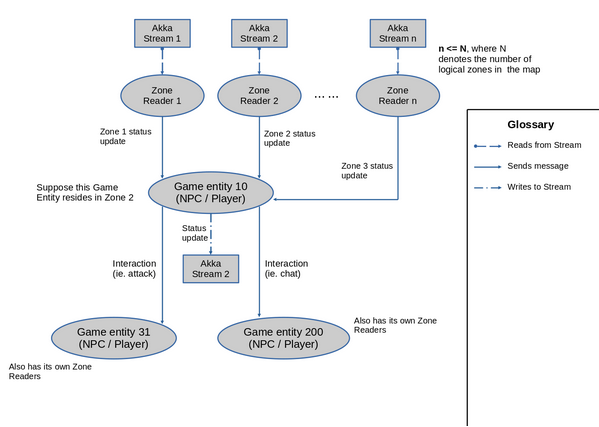
\includegraphics[width=0.5\textwidth]{../assets/architecture.png}
    \caption{Diagrama de arquitectura propuesta utilizando el modelo de actores y streams}
\end{figure}

Para solucionar el problema mencionado anteriormente, planteamos desde el diseño tener al juego 
dividido en “secciones” o “niveles” (que no necesariamente sean niveles o zonas físicas distintas) 
donde los actores correspondientes a cada entidad únicamente conocerán (y por tanto podrán interactuar) 
con actores de su misma zona o zonas adyacentes. Esto nos acota la carga de mensajes sobre cada actor, 
ya que si cada actor pudiera comunicarse con cualquier otro, terminaremos teniendo un carga de 
N cuadrado, donde N denota a los actores del juego (las entidades).

Los entidades podrán interactuar entre ellas a través de los mensajes entre los actores, 
sin embargo optamos por utilizar \textit{Akka Streams} para todo lo que sea actualizaciones globales 
del estado para evitar el problema de saturar las mailboxes de los actores ante eventos muy 
recurrentes, como es el claro ejemplo de las actualizaciones de las posiciones de los actores. 
La idea es que cada entidad tendrá asociada un actor por zona del juego encargado de leer del 
Stream de esa zona y agrupar varias de las actualizaciones de estado más generales (en forma de batch) 
y enviar por mensaje al actor principal de la entidad esas actualizaciones. 
Así disminuimos considerablemente la cantidad de mensajes que tiene que procesar cada actor 
principal de la entidad y además aprovechamos el mecanismo de back pressure que Akka Stream 
provee transparentemente. Cada actor principal de la entidad entonces envía sus actualizaciones 
generales (por ejemplo la posición) a través del Stream de la zona en la que reside, para que 
sea consumida por los actores de las demás entidades.



\subsection{Backend: servidor distribuido Akka}
\index{Desarrollo}

\subsubsection{Introducción a Akka}

\subsubsection{Arquitectura}

\subsubsection{Diagramas}

\subsubsection{Mensajes de Kafka}


\subsection{Frontend: cliente Godot}

\noindent \textit{Godot} es un motor para desarrollar videojuegos, argentino, gratuito y de código abierto. 
Este motor brinda distintas herramientas para desarrollar aplicaciones interactivas, como por ejemplo 
interfaces gráficas, gráficos 2D y 3D, input del usuario con distintos periféricos, control de audio, 
lógica de físicas y colisiones, conectividad a través de la red, entre muchas otras.
Además de permitir desarrollar para múltiples plataformas, permite programar scripts exponiendo una 
API orientada a objetos en los lenguajes C++, C\# e incluso GDScript, un lenguaje propio de Godot.

El motor ofrece una amplia colección de Nodos, que son los componentes básicos que se utilizan para 
construir Escenas, que a su vez pueden ser sub-nodos de otras escenas. Los Nodos pueden ser desde un 
simple botón (\textbf{Button}) hasta un cuerpo con lógica de físicas y colisiones tridimensionales 
(\textbf{PhysicsBody3D}) e incluso un \textbf{AnimationPlayer} que se encarga de manejar animaciones, 
es decir, una secuencia de imágenes o \textit{Sprites}.

Otro feature importante de Godot es el uso de señales (\textit{signals}) para comunicar eventos entre nodos.
Un Nodo cualquiera o una Escena personalizada pueden emitir \textit{signals} con un nombre específico 
(incluso con parámetros) para que otros Nodos o Escenas se suscriban a dicha señal. Al suscribirse, los 
Nodos receptores definen un handler (comúnmente nombrado \textit{\_on\_node\_signal\_name}) para manejar 
la señal recibida. De esta forma se pueden crear escenas compuestas de múltiples Nodos distintos, con 
comportamiento más complejo, pero sin acoplar todos los nodos que necesiten comunicarse entre sí.

La filosofía del diseño de Godot es construir escenas reutilizables usando nodos. A estas escenas y 
nodos se les puede agregar comportamiento con \textit{scripts}. Con la composición y jerarquía de los Nodos, 
se puede construir una lógica de juego que es clara y fácil de entender.

\subsubsection{Estructura de proyecto}

\noindent Para este proyecto, definimos una Escena \textbf{Main} donde instanciamos las escenas del juego necesarias 
a medida que sean requeridas. Por ejemplo, los niveles propiamente dichos no se instancian al iniciar el 
juego, sino después de que el jugador se haya conectado al servidor. De esta forma, encapsulamos todas las 
escenas activas en un mismo lugar y no desperdiciamos recursos instanciando todas las escenas a la vez.

Además hacemos uso de los \textbf{Autoloads} de Godot, que funcionan igual que el patrón \textbf{Singleton}, 
para ciertas Escenas o scripts que son necesarios en un scope global. Por ejemplo, para el manejo, carga 
y borrado de escenas, hacemos uso de un \textbf{SceneManager}, que es un script Autoload que permite 
transicionar entre niveles dentro del juego. En general, se implementaron Singletons de tipo \textit{Manager}
para acceder a distintos comportamientos y configuraciones globales (información del jugador, cambio de 
escenas, control del audio, entre otros).

\subsubsection{Comunicación con el servidor}

\noindent Al comienzo del proyecto, un posible limitante de usar Godot eran las herramientas que podía ofrecer 
el motor para la conectividad con el servidor, ya sea UDP, TCP o incluso HTTP. 
Para nuestro beneficio, Godot provee distintas APIs para conectividad que cumplen los requisitos
de los protocolos antes mencionados. En nuestro caso, decidimos usar el protocolo TCP por sus características:
\begin{itemize}
    \item Handshake con el Servidor
    \item Conexión mantenida con el Servidor
    \item Garantía de recepción de todos los paquetes enviados
    \item \textit{Flow Control}
\end{itemize}

Luego, definimos nuestras propias clases \textit{wrapper} para establecer la conexión al servidor y el 
manejo de mensajes. 

Para la recepción implementamos un \textbf{ServerConsumer} que se encarga de recibir los paquetes 
del Servidor, parsea el mensaje completo (ver sección Protocol buffers) y según qué mensaje recibió, 
invoca al \textit{handler} correspondiente para actualizar el estado del juego del lado del Cliente.

Es análogo el envío de mensajes en el sentido desde el Cliente hacia el Servidor: algún input de un 
usuario dispara una \textit{signal} que el \textbf{ServerProducer} recibe, este se encarga de crear 
el mensaje correspondiente con los parámetros correctos, lo serializa y envía los paquetes de bytes 
al Servidor a través de la conexión TCP.

\subsection{Comunicación entre cliente y servidor}

\subsubsection{Protocol buffers}

\noindent La comunicación entre Cliente y Servidor requirió que definamos un protocolo de mensajes propio para 
el envío de acciones del Cliente y las correspondientes actualizaciones del Servidor.
Para esto no solo necesitamos definir un protocolo de mensajes, sino además que sea rápido y eficiente, 
para mantener al mínimo la latencia entre mensajes.
Es por esto que decidimos usar \textit{Protocol buffers} (o \textit{protobufs}). Los 
\textit{Protocol buffers} son un mecanismo para serializar datos estructurados, ajeno completamente 
a algún lenguaje. El propósito es definir los mensajes del protocolo una sola vez y reutilizarlos 
tanto en el Cliente como el Servidor.
Por ejemplo, veamos el siguiente mensaje que definimos para el movimiento de un usuario:
\begin{verbatim}
    message PBPlayerVelocity {
        required float x = 1;
        required float y = 2;
    }

    message PBPlayerPosition {
        required float x = 1;
        required float y = 2;
    }

    message PBPlayerMovement {
        required PBPlayerVelocity velocity = 1;
        required PBPlayerPosition position = 2;
    }
\end{verbatim}

El mensaje que el Cliente enviará es \textbf{PBPlayerMovement}, que se compone de otros dos mensajes: 
\textbf{PBPlayerVelocity} y \textbf{PBPlayerPosition}, ambos vectores bidimensionales representados 
por sus coordenadas en \textbf{x} e \textbf{y}. De esta forma cuando el usuario controla y mueve a 
su personaje, el Cliente se lo comunica al Servidor creando una instancia de \textbf{PBPlayerMovement} 
con los valores correspondientes, serializandolo y finalmente enviandolo.


La totalidad de los mensajes que definimos en nuestro protocolo está en el Anexo \ref{apendix:protobuf}

\begin{figure}[htbp]
    \centering
    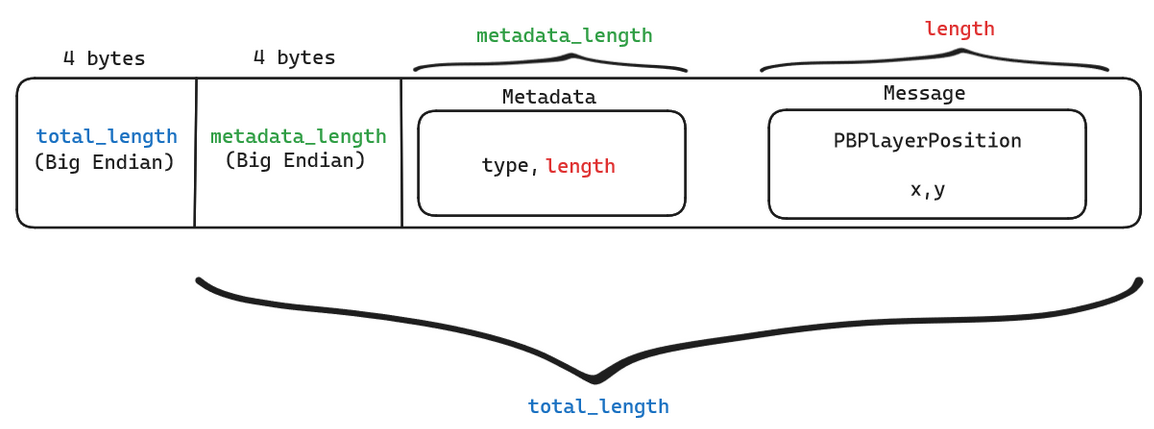
\includegraphics[width=1.0\textwidth]{../assets/protobuf.png}
\end{figure}

\subsubsection{Lógica del juego: movimiento y colisiones}
\noindent Otro de nuestros problemas iniciales fue decidir cómo implementaríamos el movimiento del 
jugador. Al tratarse de un juego online, lo ideal era que la lógica fuera mayormente implementada del 
lado del servidor y así garantizar que los jugadores no pudieran realizar movimientos prohibidos, como 
ir a zonas que no estuvieran permitidas u obtener algún tipo de ventaja. Con este acercamiento del 
problema, Godot no debería hacer más que enviar los inputs de la dirección a la que se desea mover el 
jugador del jugador, y dejar que el 
servidor se encargara de verificar que se tratase de un input válido, calcular el efecto de este 
input en la posición y enviar a Godot la nueva dirección para que se viera reflejada en el juego.

Este acercamiento sirvió en un inicio donde el juego era un prototipo donde no teníamos definidos 
mapas con un perímetro definido, sin embargo empezaron a verse las faltas en esta solución cuando 
se comenzó a implementar las colisiones del jugador con los mapas y los objetos dentro de sus límites.

Se decidió ceder la mayor parte de la lógica del movimiento a Godot debido a que este provee 
su propio sistema de colisiones, aprovechando las herramientas que provee sin reinventar un sistema 
colisiones. Este acercamiento nos hacía renunciar a que el input fuera 
verificado con cada movimiento, pero facilitaba de forma significativa la implementación del 
movimiento y las colisiones. Debido a que nuestro juego no muestra ninguna ventaja competitiva 
en la modificación del movimiento del jugador, decidimos perder parte de las verificaciones en 
favor a la facilidad de desarrollo provista por Godot.

% algoritmos de colisiones son resolubles en el backend, era reiventar la rueda, ya tenemos godot <3
% y no sabíamos cómo iba a ir el tema de performance.

\subsubsection{Juego de cartas: Truco}
\noindent A modo de muestra del tipo de funcionalidades que se pueden desarrollar en conjunto de 
Godot y el modelo de actores, hemos implementado el juego de cartas \textbf{Truco}, específicamente 
en su versión argentina.

Al igual que con el movimiento del jugador y las colisiones, debimos decidir qué 
responsabilidades recaerían tanto para el frontend como para el backend. En la sección 
sobre el movimiento del jugador, concluímos que no existía una importante necesidad de 
validar cada movimiento del jugador, pero el caso de un minijuego como el Truco es distinto. 
En el movimiento, que los demás jugadores vean a otro jugador en una posición incorrecta es 
corregible, momentáneo e insignificante, pero en el Truco, que un jugador presencie una acción 
incorrecta es inaceptable debido a que cada acción realizada por un jugador afecta el flujo del juego.

Para poder mantener la coherencia y la integridad de una partida de Truco, se decidió dejar 
la responsabilidad del manejo de flujo y las verificaciones al backend, mientras que el 
frontend tiene la responsabilidad de mostrarle al jugador todo lo que el backend dicte, 
como por ejemplo las cartas en su mano, las jugadas de su adversario y los cantos disponibles. 
El frontend también posee la responsabilidad de ofrecerle una buena jugabilidad al jugador, 
por lo que la interfaz de juego fue diseñada con estas intenciones. Implementamos un método 
de movimiento para jugar las cartas denominado “drag and drop” para que el jugador pueda 
arrastrar las cartas en caso de que desee jugarlas o volver a colocarla en la mano con tan 
solo volver a arrastrarla a su zona original y una interfaz que muestre los cantos disponibles; 
un cartel que aparezca para avisarle al jugador que su oponente realizó un canto y que luego 
desaparezca, indicadores de a qué jugador le corresponde realizar una jugada, entre otras cosas.
